\documentclass[11pt]{article}
\usepackage[margin=1in]{geometry}
\usepackage[T1]{fontenc}
\usepackage[utf8]{inputenc}
\usepackage[expansion=false]{microtype}
\usepackage{amsmath,amssymb,amsthm}
\usepackage{amsfonts}
\theoremstyle{plain}
\newtheorem{lemma}{Lemma}[section]
\usepackage{natbib}
\setcitestyle{authoryear,open={(},close={)}}
\usepackage{graphicx}
\usepackage{booktabs}
\usepackage{hyperref}
\usepackage{cleveref}
\usepackage{float}  

\hypersetup{
    colorlinks=true,
    linkcolor=blue,
    citecolor=blue,
    urlcolor=blue,
    pdftitle={A Unified Framework for Adjusting Effective Time to Expiration in TWAP- and VWAP-Settled Options},
    pdfauthor={Evan Semet}
}


\title{A Unified Framework for Adjusting Effective Time to Expiration in TWAP- and VWAP-Settled Options}
\author{Evan Semet}
\date{May 4, 2025}

\begin{document}

\maketitle

\begin{abstract}
Derivatives settled on average-price benchmarks such as Time-Weighted Average Price (TWAP) and Volume-Weighted Average Price (VWAP) introduce unique valuation challenges: while discounting occurs over the full contractual horizon, volatility exposure is reduced due to averaging effects. We derive from first principles expressions for the variance of the average log-price for both TWAP and VWAP settlements, considering pre- and intra-window regimes where applicable. We map these variances to an equivalent single-period time-to-expiration (TTE), $T_{\mathrm{eff}}$, and embed these adjustments into Black–Scholes and Black–76 formulas, providing a computationally efficient method for pricing these contracts. For VWAP, we provide an explicit closed-form analysis using a power-law volume profile ($v(s) \propto s^\alpha$, where $s$ is time since window start) over a final averaging window $[T-t_w, T]$. We introduce formal lemmas with detailed proofs, drawing parallels to the treatment of Asian options. This framework addresses significant practical issues related to interpreting implied volatility dynamics near expiry for average-settled options.
\end{abstract}

\section{Introduction}
\label{sec:introduction}

Financial derivatives are increasingly settled against average price benchmarks rather than a single price at maturity. Common examples include options settling on the Time-Weighted Average Price (TWAP), which computes the arithmetic average of the underlying spot price over a fixed pre-close window, or the Volume-Weighted Average Price (VWAP), which weights prices by traded volume over a chosen interval \citep[see e.g.,][for benchmark definitions]{kissell2013science}. While these benchmarks are widely used in execution algorithms and trade reporting, the direct implications for derivative pricing, particularly regarding the adjustment of standard option pricing model inputs, remain relatively underexplored in accessible literature and can lead to significant practical challenges for traders and risk managers.

Standard option pricing models, such as Black-Scholes \citep{blackscholes1973pricing, merton1973theory} or Black-76 for futures options \citep{black1976pricing}, assume a point-in-time settlement at maturity $T$. The uncertainty, driven by volatility $\sigma$, accumulates over the time-to-expiration $\tau = T-t$, contributing $\sigma^2 \tau$ to the variance of the log-price. However, when the settlement price is an average over an interval (like the final 30 minutes for a TWAP), this averaging process dampens the price fluctuations, effectively reducing the variance exposure attributed to the underlying's volatility as settlement approaches.

Ignoring this effect leads to practical problems. If market participants price these options correctly (implicitly accounting for the averaging) but traders analyze them using standard models with calendar time $\tau$, the implied volatility backed out from market prices will appear to decay rapidly and non-intuitively as the averaging window is entered, even if the underlying's true volatility is constant. This makes comparing implied volatility levels across different contract expiries, or across exchanges with slightly different settlement rules or windows, extremely difficult. Gauging true volatility premiums becomes obscured by these contract-specific artifacts. Furthermore, the resulting term structure of implied volatility and derived forward volatilities exhibit kinks and apparent decays that are hard to interpret or model consistently. Conversely, if market prices \textit{fail} to account for the averaging, applying a theoretically correct model (like the one developed here) would imply unrealistic spikes in effective volatility near settlement.

This paper addresses these issues by developing a framework based on an "effective" time-to-expiration, $T_{\mathrm{eff}}$. We ask:
\begin{enumerate}
    \item How can we quantify the variance reduction from averaging and map it to an adjusted time parameter $T_{\mathrm{eff}}$?
    \item How can $T_{\mathrm{eff}}$ be integrated into standard Black-Scholes/Black-76 models to correctly price TWAP/VWAP-settled options while maintaining consistency in volatility interpretation?
\end{enumerate}
We derive $T_{\mathrm{eff}}$ for both TWAP and VWAP settlements (using a power-law volume profile example for the latter) based on the variance of the average log-price. We demonstrate how substituting $T_{\mathrm{eff}}(\tau)$ for $\tau$ specifically in the terms related to volatility ($\sigma^2 T_{\mathrm{eff}}$ and $\sigma \sqrt{T_{\mathrm{eff}}}$) within standard formulas, while retaining calendar time $\tau$ for discounting ($e^{-r\tau}$) and drift terms ($r\tau$, $(r-q)\tau$), resolves the inconsistencies.

The primary benefit of this $T_{\mathrm{eff}}$ framework is that it provides a consistent and practical way to handle average-price settlements. It allows practitioners to use standard, observable underlying volatility ($\sigma$) as input, with the averaging effect contained within $T_{\mathrm{eff}}$. This normalization clarifies risk assessment, simplifies comparisons across contracts and venues, stabilizes implied volatility interpretation near expiry, and offers a computationally efficient alternative to simulation-based pricing for these common derivatives.

\section{Literature Review and Distinction from Asian Options}
\label{sec:literature}

\subsection{Asian Options vs. Average-Price Settlement Mechanisms}
The concept of options depending on average prices is most famously associated with Asian options. The defining characteristic of an Asian option is that its \textit{payoff function itself} is based on the average underlying price over a specified period, such as $\max(S_{\mathrm{Avg}} - K, 0)$ or $\max(K - S_{\mathrm{Avg}}, 0)$ where $S_{\mathrm{Avg}}$ is computed over part or all of the option's life \citep{kemna1990pricing, hull2006options}. The extensive literature on Asian options primarily focuses on the challenges of pricing this specific payoff structure. A key difficulty arises because the arithmetic average of log-normally distributed variables (like $S(t)$ under GBM) does not follow a log-normal distribution, complicating the derivation of closed-form solutions. Therefore, research often involves developing accurate analytic approximations, or employing numerical techniques like Monte Carlo simulation or solving partial differential equations (PDEs).

Our study, while mathematically related through the analysis of averaged prices, addresses a different problem. We focus on options that may have a standard European payoff structure (e.g., settlement based on $\max(S_T - K, 0)$ or $\max(F_T - K, 0)$) but where the \textit{final underlying price} ($S_T$ or $F_T$) used for settlement is determined by an \textit{average price fixing mechanism}, such as TWAP or VWAP, over a specific window leading up to maturity. The core impact we analyze is how this \textit{settlement procedure} affects the \textit{effective variance} experienced by the option holder, particularly near expiry.

Our objective is not to derive a new pricing formula for a fundamentally different payoff, but rather to provide a practical adjustment to the \textit{inputs} of existing, standard models (Black-Scholes, Black-76). We achieve this by calculating the variance reduction due to the averaging mechanism and encapsulating it within an effective time-to-expiration, $T_{\mathrm{eff}}$. This $T_{\mathrm{eff}}$ then replaces the standard time $\tau$ \textit{only} in the volatility-related terms of the standard formulas. The payoff structure itself and the discounting over the calendar time $\tau$ remain unchanged from the standard European option context. Although calculating the variance of the average log-price employs similar mathematical tools as used in Asian option analysis \citep[e.g.,][]{kemna1990pricing}, our goal is distinct: to offer a computationally efficient adjustment factor ($T_{\mathrm{eff}}$) that allows practitioners to continue using familiar pricing frameworks while correctly accounting for the variance-dampening effect of TWAP/VWAP settlement fixings. This maintains the tractability of closed-form solutions and provides a clear interpretation of implied volatility.

\subsection{TWAP/VWAP Benchmarks}
TWAP and VWAP are standard execution benchmarks in algorithmic trading \citep{kissell2013science}. VWAP, in particular, aims to capture the average price at which most volume traded. The specific calculation interval and volume profiles used can vary significantly in practice. While models exist for optimal execution relative to these benchmarks \citep[e.g.,][]{almgren2001optimal}, their use as the \textit{settlement price} for derivatives and the resulting pricing implications via effective variance adjustment is less commonly detailed.

\section{Mathematical Model}
\label{sec:model}

Assume under the risk-neutral measure $\mathbb{Q}$ that the underlying asset price $S(t)$ follows geometric Brownian motion (GBM), the foundational model for option pricing \citep{blackscholes1973pricing, merton1973theory, hull2006options}:
\begin{equation} \label{eq:gbm}
    dS(t) = r S(t)\,dt + \sigma S(t)\,dW^{\mathbb{Q}}(t),
\end{equation}
where $r$ is the constant continuously compounded risk-free rate, $\sigma$ is the constant volatility of the underlying asset price, and $W^{\mathbb{Q}}(t)$ is a standard Brownian motion under the measure $\mathbb{Q}$. We omit the superscript $\mathbb{Q}$ for brevity in subsequent notation. For assets paying a continuous dividend yield $q$, the drift term becomes $(r-q)S(t)\,dt$.

\subsection{TWAP Spot Price Definition}
Let $T$ denote the contract maturity date/time and $t_w$ the length of the averaging window immediately preceding maturity ($0 < t_w \le T$). The Time-Weighted Average Price (TWAP) used for settlement at $T$ is defined as the continuous arithmetic average over the interval $[T - t_w, T]$:
\begin{equation} \label{eq:twap_def}
  S_{\mathrm{TWAP}} = \frac{1}{t_w} \int_{T - t_w}^{T} S(u) \,du.
\end{equation}

\subsection{VWAP Spot Price Definition}
Let the Volume-Weighted Average Price (VWAP) be calculated over a specific interval $[T_1, T_2]$ (common choices include the full period $[0, T]$ or a window $[T-t_w, T]$). Let $v(u)$ be the non-negative function representing the rate of volume traded at time $u$ within this interval. The VWAP spot price is the price weighted by volume \citep[see e.g.,][]{kissell2013science}:
\begin{equation} \label{eq:vwap_def_general}
  S_{\mathrm{VWAP}} = \frac{\int_{T_1}^{T_2} v(u) S(u)\,du}{\int_{T_1}^{T_2} v(u)\,du}.
\end{equation}
We define the total volume over the interval as $V = \int_{T_1}^{T_2} v(u)\,du$. Assuming $V > 0$, we can define a normalized volume weight function $w(u) = v(u) / V$, which satisfies $\int_{T_1}^{T_2} w(u)\,du = 1$. The VWAP definition simplifies to:
\begin{equation} \label{eq:vwap_def_normalized}
  S_{\mathrm{VWAP}} = \int_{T_1}^{T_2} w(u) S(u)\,du.
\end{equation}
This formulation highlights VWAP as a weighted average, similar to TWAP but with potentially non-uniform weights.

\section{Variance Analysis}
\label{sec:variance}

The core idea of our framework is to map the variance of the average settlement price (or, more tractably, the average log-price under GBM) to an equivalent variance for a standard option, $\sigma^2 T_{\mathrm{eff}}$. This allows us to isolate the impact of the averaging mechanism into a single adjusted time parameter, $T_{\mathrm{eff}}$. We use the variance of the average log-price, $\mathrm{Var}[\int w(u) \ln S(u) du]$, as it is analytically tractable under the GBM assumption and forms the basis for common approximations for Asian option pricing \citep[e.g.,][]{kemna1990pricing}. The resulting effective time $T_{\mathrm{eff}}$ replaces the standard TTE $\tau = T-t$ in the volatility term $\sigma\sqrt{\tau}$ within the Black-Scholes/Black-76 formulas, while the discounting term $e^{-r\tau}$ continues to use the actual calendar time $\tau$.

\subsection{TWAP Variance}
\label{sec:twap_variance}

Under GBM, the log-price $\ln S(t)$ follows a Brownian motion with drift. Relative to time 0, $\ln S(u) \sim \mathcal{N}((r-\sigma^2/2)u, \sigma^2 u)$, and the covariance is $\mathrm{Cov}[\ln S(u),\ln S(v)] = \sigma^2 \min(u,v)$. The variance of the average log-price $\bar{L}_{TWAP} = \frac{1}{t_w} \int_{T-t_w}^T \ln S(u) du$ relative to time 0 can be shown to be $\sigma^2 (T-t_w) + \sigma^2 t_w/3$. The calculation involves integrating the covariance function:
\begin{align*}
    \mathrm{Var}_0[\bar{L}_{TWAP}] &= \frac{1}{t_w^2} \mathrm{Var}_0\left[ \int_{T-t_w}^T \ln S(u) du \right] \\
    &= \frac{1}{t_w^2} \int_{T-t_w}^T \int_{T-t_w}^T \mathrm{Cov}[\ln S(u), \ln S(v)] du dv \\
    &= \frac{\sigma^2}{t_w^2} \int_{T-t_w}^T \int_{T-t_w}^T \min(u,v) du dv.
\end{align*}
Let $u' = u - (T-t_w)$ and $v' = v - (T-t_w)$, ranging from $0$ to $t_w$. Then $\min(u,v) = \min(u'+T-t_w, v'+T-t_w) = \min(u',v') + T-t_w$. The integral becomes:
\begin{align*}
    &\int_{0}^{t_w} \int_{0}^{t_w} (\min(u',v') + T-t_w) du' dv' \\
    &= \int_{0}^{t_w} \int_{0}^{t_w} \min(u',v') du' dv' + \int_{0}^{t_w} \int_{0}^{t_w} (T-t_w) du' dv' \\
    &= \frac{t_w^3}{3} + (T-t_w)t_w^2.
\end{align*}
(The result $\int_0^\tau \int_0^\tau \min(s,p) ds dp = \tau^3/3$ is standard).
Thus,
\begin{align*}
\mathrm{Var}_0[\bar{L}_{TWAP}] &= \frac{\sigma^2}{t_w^2} \left( \frac{t_w^3}{3} + (T-t_w)t_w^2 \right) \\
&= \sigma^2 \frac{t_w}{3} + \sigma^2(T-t_w).
\end{align*}
For pricing an option at time $t < T$, we need the conditional variance $\mathrm{Var}_t[\dots]$ of the average over the remaining time until settlement, $\tau = T-t$. The calculation depends on whether the valuation time $t$ is before or within the averaging window $[T-t_w, T]$.

\begin{lemma}[TWAP Pre-Window Regime] \label{lem:pre_window}
If the valuation time $t$ is before the averaging window starts, i.e., $t < T - t_w$ (which is equivalent to $\tau > t_w$), the conditional variance of the average log-price relevant for pricing is:
\[
  \mathrm{Var}_{t, \mathrm{pre}}^{\mathrm{TWAP}}[\text{AvgLogPrice}] = \sigma^2(\tau - t_w) + \frac{\sigma^2 t_w}{3}.
\]
\end{lemma}
\begin{proof}
  The logic relies on the tower property of conditional expectation and variance. Variance accumulates normally as $\sigma^2 \times (\text{time})$ until the start of the window at $T-t_w$. The remaining variance comes from the average over the window $[T-t_w, T]$, whose total variance contribution (conditional on time $T-t_w$) is known to be $\sigma^2 t_w / 3$. See standard derivations for variance of integrated Brownian motion.
\end{proof}

\begin{lemma}[TWAP Intra-Window Regime] \label{lem:intra_window}
If the valuation time $t$ is within the averaging window, i.e., $T - t_w \le t < T$ (which is equivalent to $0 < \tau \le t_w$), the conditional variance relevant for pricing, arising from the remaining averaging interval $[t, T]$, is:
\[
  \mathrm{Var}_{t, \mathrm{intra}}^{\mathrm{TWAP}}[\text{AvgLogPrice}] = \frac{\sigma^2 \tau^3}{3\,t_w^2}.
\]
\end{lemma}
\begin{proof}
  We require the conditional variance of the remaining part of the average, given information $\mathcal{F}_t$:
  \[
  \mathrm{Var}_t\left[ \frac{1}{t_w} \int_{t}^{T} \ln S(u) \,du \right].
  \]
  Under GBM, $\ln S(u) = \ln S(t) + (r-\sigma^2/2)(u-t) + \sigma (W(u)-W(t))$. The conditional variance arises solely from the stochastic integral involving the future Brownian motion increments:
  \[
  \mathrm{Var}_t\left[ \frac{\sigma}{t_w} \int_{t}^{T} (W(u)-W(t)) \,du \right].
  \]
  Let $s = u-t$, so $u = t+s$, and $du=ds$. Let $B(s) = W(t+s) - W(t)$, which is a standard Brownian motion starting at $B(0)=0$. The remaining time is $\tau = T-t$. The expression becomes:
  \begin{align*}
    \frac{\sigma^2}{t_w^2} &\mathrm{Var}\left[ \int_0^{\tau} B(s) \,ds \right] \\
    &= \frac{\sigma^2}{t_w^2} E\left[ \left( \int_0^{\tau} B(s) \,ds \right)^2 \right] \\
    &= \frac{\sigma^2}{t_w^2} \int_0^{\tau} \int_0^{\tau} E[B(s) B(p)] \,ds\,dp \\
    &= \frac{\sigma^2}{t_w^2} \int_0^{\tau} \int_0^{\tau} \min(s, p) \,ds\,dp \\
    &= \frac{\sigma^2 \tau^3}{3\,t_w^2}.
  \end{align*}
  The result $\int_0^\tau \int_0^\tau \min(s,p) ds dp = \tau^3/3$ is a standard result for integrated Brownian motion variance.
\end{proof}

Mapping these conditional variances to an effective TTE by setting $\sigma^2 T_{\mathrm{eff}} = \mathrm{Var}_t[\text{AvgLogPrice}]$, we get:
\begin{equation} \label{eq:tte_eff_twap}
  T_{\mathrm{eff}}^{\mathrm{TWAP}}(\tau, t_w) =
  \begin{cases}
    (\tau - t_w) + \frac{t_w}{3}, & \text{if } \tau > t_w \text{ (Pre-window)}, \\
    \frac{\tau^3}{3\,t_w^2},       & \text{if } 0 < \tau \le t_w \text{ (Intra-window)}.
  \end{cases}
\end{equation}
Note that the function $T_{\mathrm{eff}}^{\mathrm{TWAP}}(\tau, t_w)$ is continuous at the boundary $\tau = t_w$, where both expressions evaluate to $t_w/3$.

\subsection{VWAP Variance}
\label{sec:vwap_variance}

For a general VWAP settlement over $[T_1, T_2]$ with normalized volume weight function $w(u)$, the variance of the weighted average log-price relative to time 0 is found by integrating the covariance function:
\begin{align}
  \mathrm{Var}_0&\left[ \int_{T_1}^{T_2} w(u) \ln S(u) \,du \right] \nonumber \\
  &= \int_{T_1}^{T_2} \int_{T_1}^{T_2} w(u) w(v) \mathrm{Cov}[\ln S(u), \ln S(v)] \,du\,dv \nonumber \\
  &= \sigma^2 \int_{T_1}^{T_2} \int_{T_1}^{T_2} w(u) w(v) \min(u,v)\,du\,dv. \label{eq:vwap_var0_general}
\end{align}
For pricing at time $t$ where $T_1 \le t < T_2$, the relevant conditional variance depends on the remaining integral from $t$ to $T_2$. Let $\tau_2 = T_2 - t$ be the time remaining in the averaging interval. Similar to the TWAP case, the conditional variance is:
\begin{align}
  \mathrm{Var}_t&\left[ \int_{t}^{T_2} w(u) \ln S(u) \,du \right] \nonumber \\
  &= \sigma^2 \int_{0}^{\tau_2} \int_{0}^{\tau_2} w(t+s_1) w(t+s_2) \min(s_1, s_2) \,ds_1\,ds_2. \label{eq:vwap_vart_general_s}
\end{align}
where $s_1, s_2$ are time variables relative to $t$.

\subsubsection{Example: Power-Law Volume Profile over Window $[T-t_w, T]$}
\label{sec:vwap_powerlaw_window_final} % New label

We model VWAP settlement over the final window $[T-t_w, T]$ ($T_1=T-t_w, T_2=T$). We assume the volume rate follows a power law relative to the start of the window. Let $s = u - (T-t_w)$ be the time elapsed since the window started ($s \in [0, t_w]$). Assume the volume rate is $v(s) = c \cdot s^\alpha$ for $s \in (0, t_w]$, with $\alpha > -1$.

The total volume $V''$ over this window is $V'' = \int_{0}^{t_w} c s^\alpha ds = \frac{c t_w^{\alpha+1}}{\alpha+1}$. The normalized weight function relative to the start of the window is:
\begin{equation} \label{eq:powerlaw_window_weight_relative_final}
  w''(s) = \frac{v(s)}{V''} = \frac{(\alpha+1) s^\alpha}{t_w^{\alpha+1}}, \quad \text{for } s \in (0, t_w].
\end{equation}
Calculating the conditional variance using this weight function via the general principles (similar to Lemmas \ref{lem:pre_window} and \ref{lem:intra_window} but using weighted integrals) leads to a closed-form solution for the effective time $T_{\mathrm{eff}}^{\mathrm{VWAP}}$.

\begin{lemma}[VWAP Effective TTE - Window Power Law $s^\alpha$] \label{lem:vwap_tte_powerlaw_window_final}
For VWAP settlement over the window $[T-t_w, T]$ with volume profile $v(s) \propto s^\alpha$ relative to the window start time $s=u-(T-t_w)$ ($\alpha > -1$), the effective time-to-expiration $T_{\mathrm{eff}}^{\mathrm{VWAP}}$ for use in option pricing at time $t$ (with time-to-expiry $\tau = T-t$) is given by the piecewise function:
\begin{equation} \label{eq:tte_eff_vwap_piecewise_final}
  T_{\mathrm{eff}}^{\mathrm{VWAP}}(\tau, t_w; \alpha) =
  \begin{cases}
     \begin{aligned}[b]
        &(\tau - t_w) \\
        & \quad + t_w \frac{2(\alpha+1)^2}{(\alpha+2)(2\alpha+3)},
     \end{aligned}
        & \text{if } \tau > t_w \\[3ex]
     \begin{aligned}[b]
        &t_w \left[ u_\tau - \frac{2}{\alpha+2}(1-(1-u_\tau)^{\alpha+2}) \right. \\
        & \quad \left. + \frac{1}{2\alpha+3}(1-(1-u_\tau)^{2\alpha+3}) \right],
     \end{aligned}
        & \text{if } 0 < \tau \le t_w
  \end{cases}
\end{equation}
where $u_\tau = \tau/t_w$ is the remaining fraction of the window duration.
\end{lemma}
\begin{proof} (Sketch)
  The pre-window case ($\tau > t_w$) combines the linear variance accumulation $\sigma^2(\tau-t_w)$ with the total conditional variance from the full window evaluated at time $T-t_w$. The intra-window case ($0 < \tau \le t_w$) results from calculating the conditional variance over the remaining interval $[t, T]$ using the weight function \eqref{eq:powerlaw_window_weight_relative_final}. Evaluating the required double integrals involving $\min(s_1, s_2)$ and the $s^\alpha$ weighting yields the closed-form expressions presented. The constant term in the pre-window case, $t_w \frac{2(\alpha+1)^2}{(\alpha+2)(2\alpha+3)}$, is the value of the intra-window expression when $\tau=t_w$ (i.e., $u_\tau=1$), ensuring continuity.
\end{proof}

This provides an explicit analytical form for $T_{\mathrm{eff}}^{\mathrm{VWAP}}$ under this specific power-law assumption, which can be computed directly.

\textbf{Consistency Check ($\alpha=0$):}
For the special case $\alpha=0$, the volume profile $s^\alpha$ is constant, corresponding to uniform weighting (TWAP). As derived previously, substituting $\alpha=0$ into Equation \eqref{eq:tte_eff_vwap_piecewise_final} correctly yields the TWAP effective time formula \eqref{eq:tte_eff_twap}, confirming consistency.


\textbf{Limiting Cases for $\alpha$:} % Added section
It is instructive to consider the behavior of the effective time formula \eqref{eq:tte_eff_vwap_piecewise_final} in the limiting cases for the power-law exponent $\alpha$.
\begin{itemize}
    \item As $\alpha \to -1^+$: The weight function $w''(s) \propto s^\alpha$ becomes increasingly concentrated near the start of the window ($s=0$). In the limit, this corresponds to all volume executing instantaneously at the beginning of the window ($t=T-t_w$). Examining the limits of the terms in \eqref{eq:tte_eff_vwap_piecewise_final}, we find that $T_{\mathrm{eff}}^{\mathrm{VWAP}}(\tau, t_w; \alpha) \to \max(0, \tau-t_w)$. Intuitively, if the VWAP price is effectively determined at the exact start of the window, there is no remaining uncertainty attributable to the window itself.
    \item As $\alpha \to \infty$: The weight function $w''(s) \propto s^\alpha$ becomes increasingly concentrated near the end of the window ($s=t_w$). In the limit, this corresponds to all volume executing instantaneously at the exact end of the window ($t=T$). In this scenario, the VWAP price becomes identical to the spot price $S(T)$. Examining the limits of the terms in \eqref{eq:tte_eff_vwap_piecewise_final}, we find that $T_{\mathrm{eff}}^{\mathrm{VWAP}}(\tau, t_w; \alpha) \to \tau$ for all $\tau > 0$. Intuitively, if the settlement price is just the spot price at maturity $T$, the averaging effect vanishes, and the effective time should revert to the actual time-to-expiration $\tau$.
\end{itemize}
These limiting behaviors align with financial intuition regarding front-loaded and back-loaded volume profiles within the averaging window.




\subsection{Illustration of Effective Time Behavior}
\label{sec:Teff_illustration}
The derived effective time adjustments significantly alter the perceived time-to-expiration used for volatility scaling. \Cref{fig:Teff_vs_tau} visually compares the calculated $T_{\mathrm{eff}}(\tau)$ for both TWAP ($\alpha=0$) and various VWAP scenarios (based on the closed-form formulas \cref{eq:tte_eff_vwap_piecewise_final} with $\alpha \neq 0$) against the standard calendar time $\tau$. The plot highlights the reduction in effective time due to averaging, particularly as expiry approaches within the averaging window.


\begin{figure}[H]
    \centering
    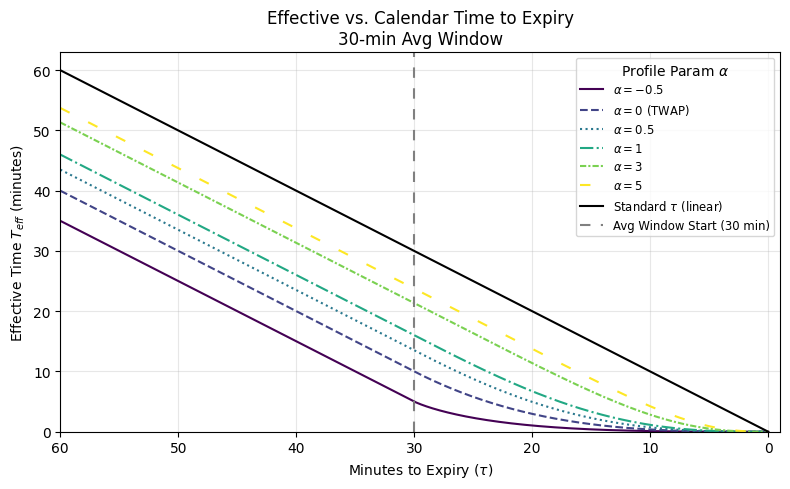
\includegraphics[width=0.5\textwidth]{png1.png}
    \caption{Effective time $T_{\mathrm{eff}}(\tau)$ vs. calendar time $\tau$ for TWAP ($\alpha=0$) and VWAP ($\alpha \neq 0$) settlement over a 30-minute window, compared to standard linear time. Assumes VWAP uses the power-law $s^\alpha$ profile over the window, evaluated using \cref{eq:tte_eff_vwap_piecewise_final}.}
    \label{fig:Teff_vs_tau}
\end{figure}



\section{Pricing Implementation}
\label{sec:implementation}

The utility of the $T_{\mathrm{eff}}$ framework lies in its straightforward application within standard option pricing formulas. To price a European option expiring at $T$ with TWAP or VWAP settlement using the Black-Scholes (for options on assets paying no or continuous dividends) or Black-76 (for options on futures) formula, we modify the standard inputs according to a simple rule:

\begin{enumerate}
    \item Calculate the appropriate $T_{\mathrm{eff}}(\tau)$ based on the settlement mechanism (e.g., \cref{eq:tte_eff_twap} for TWAP, \cref{eq:tte_eff_vwap_piecewise_final} for the windowed power-law VWAP) for the current time-to-expiration $\tau = T-t$.
    \item In the standard Black-Scholes or Black-76 formula, replace the calendar time $\tau$ with $T_{\mathrm{eff}}(\tau)$ \textbf{only} where it appears multiplying the volatility $\sigma$ or variance $\sigma^2$.
    \item Crucially, the discounting factor $e^{-r\tau}$ must continue to use the full calendar time $\tau$ to reflect the time value of money over the entire period $t$ to $T$.
    \item Similarly, any drift component related to the risk-free rate $r$ and dividend yield $q$, specifically the term $(r-q)\tau$ that appears in the $d_1$ calculation when using the spot price $S_t$ in Black-Scholes, should also retain the calendar time $\tau$.
\end{enumerate}

Let's illustrate with the Black-Scholes formula for a European call option on an asset $S_t$ with continuous dividend yield $q$. The standard formula uses $d_1^{\mathrm{std}} = [\ln(S_t/K) + (r - q + \frac{1}{2}\sigma^2)\tau] / (\sigma \sqrt{\tau})$ and $d_2^{\mathrm{std}} = d_1^{\mathrm{std}} - \sigma \sqrt{\tau}$. Applying our adjustment rule for an average-settled option $C_{\mathrm{Avg}}$:
\begin{equation}
  C_{\mathrm{Avg}} = S_t e^{-q\tau} N(d_1) - K e^{-r\tau} N(d_2)
\end{equation}
where the adjusted $d_1$ and $d_2$ become:
\begin{align}
  d_1 &= \frac{\ln(S_t/K) + (r - q)\tau + \frac{1}{2}\sigma^2 T_{\mathrm{eff}}(\tau)}{\sigma \sqrt{T_{\mathrm{eff}}(\tau)}} \label{eq:d1_spot_adjusted_revised} \\
  d_2 &= d_1 - \sigma \sqrt{T_{\mathrm{eff}}(\tau)} \label{eq:d2_spot_adjusted_revised}
\end{align}
Note how $(r-q)\tau$ retains $\tau$, while $\frac{1}{2}\sigma^2\tau$ becomes $\frac{1}{2}\sigma^2 T_{\mathrm{eff}}(\tau)$ and the denominator uses $\sigma \sqrt{T_{\mathrm{eff}}(\tau)}$. The discounting term $e^{-r\tau}$ remains unchanged.

It is often convenient to work with the forward price $F_t = S_t e^{(r-q)\tau}$. Substituting this into \cref{eq:d1_spot_adjusted_revised} simplifies the numerator: $\ln(S_t/K) + (r - q)\tau = \ln(F_t e^{-(r-q)\tau}/K) + (r - q)\tau = \ln(F_t/K)$. Thus, the $d_1$ and $d_2$ terms expressed using the forward price are:
\begin{align}
  d_1 &= \frac{\ln(F_t/K) + \frac{1}{2}\sigma^2 T_{\mathrm{eff}}(\tau)}{\sigma \sqrt{T_{\mathrm{eff}}(\tau)}} \label{eq:d1_fwd_adjusted_revised} \\
  d_2 &= d_1 - \sigma \sqrt{T_{\mathrm{eff}}(\tau)} \label{eq:d2_fwd_adjusted_revised}
\end{align}

Note that we retain the standard forward price $F_t$ (incorporating drift over $\tau$) for simplicity and tractability, focusing the adjustment on the variance term via $T_{\mathrm{eff}}$, which captures the dominant effect of the averaging settlement on option pricing and implied volatility near expiry.

The call price using the forward price is $C_{\mathrm{Avg}} = e^{-r\tau} [ F_t N(d_1) - K N(d_2) ]$.

Now, consider the Black-76 formula for a European call option on a futures contract with price $F_t$. The standard formula uses $d_1^{\mathrm{std}} = [\ln(F_t/K) + \frac{1}{2}\sigma^2 \tau] / (\sigma \sqrt{\tau})$ and $d_2^{\mathrm{std}} = d_1^{\mathrm{std}} - \sigma \sqrt{\tau}$. Applying the $T_{\mathrm{eff}}$ adjustment rule (replace $\tau$ only where it scales $\sigma$ or $\sigma^2$, keep $e^{-r\tau}$):
\begin{equation}
  C_{\mathrm{Avg}} = e^{-r\tau} \left[ F_t N(d_1) - K N(d_2) \right]
\end{equation}
where the adjusted $d_1$ and $d_2$ are precisely the same as those derived for the Black-Scholes model using the forward price.

This demonstrates that when expressed in terms of the appropriate forward or futures price $F_t$, the $T_{\mathrm{eff}}$ adjustment leads to a unified structure for the $d_1$ and $d_2$ parameters in both the Black-Scholes and Black-76 models.

This approach retains the computational tractability of the original closed-form formulas. Once $T_{\mathrm{eff}}(\tau)$ is calculated (using the analytical formulas \cref{eq:tte_eff_twap} or \cref{eq:tte_eff_vwap_piecewise_final}), the option price is obtained almost instantaneously, avoiding the need for computationally intensive Monte Carlo simulation or complex PDE solutions for pricing itself.

\section{Implications for Implied Volatility Analysis}
\label{sec:implied_vol_implications}

As highlighted in the Introduction, the $T_{\mathrm{eff}}$ framework is essential not just for pricing but also for correctly interpreting implied volatility derived from market prices of average-settled options. Failing to account for the averaging mechanism leads to apparent volatility dynamics that are artifacts of model mismatch, complicating risk management and market analysis. We illustrate this by considering two scenarios for a TWAP-settled option nearing expiry.

\subsection{Scenario 1: Correct Market Prices, Naive IV Calculation}

Assume the market correctly prices a TWAP-settled option, consistent with the $T_{\mathrm{eff}}$ model and a true underlying volatility $\sigma_{true}$. If a practitioner observes these prices but calculates implied volatility using a \textit{standard} Black-Scholes model (with calendar time $\tau$), the resulting "naive" implied volatility exhibits non-intuitive behavior. As shown in \Cref{fig:naive_iv_decay}, this naive implied volatility artificially decays as the option enters the averaging window ($\tau \le t_w$), simply because the standard model forces the variance reduction effect into the volatility parameter instead of the time parameter.

\begin{figure}[H]
    \centering
    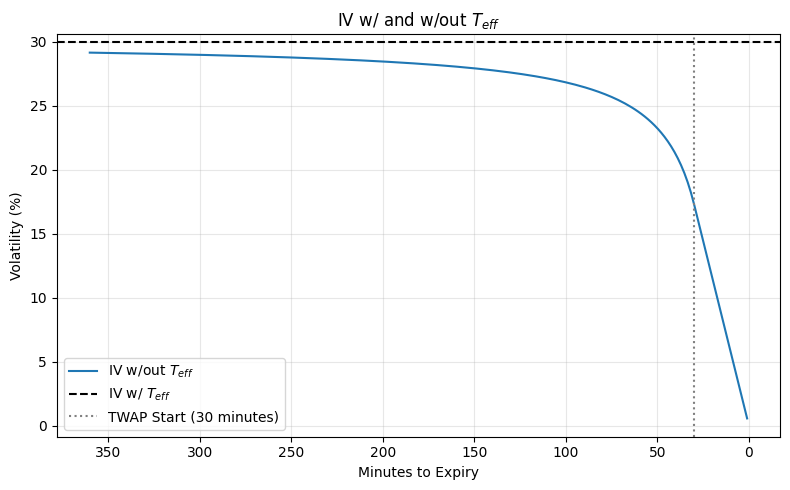
\includegraphics[width=0.5\textwidth]{png2.png}
    \caption{Apparent decay of naive implied volatility when correctly priced TWAP options are analyzed using a standard Black-Scholes model with calendar time $\tau$. The implied volatility appears to decrease within the averaging window even if true volatility is constant.}
    \label{fig:naive_iv_decay}
\end{figure}


This apparent decay distorts the term structure. \Cref{fig:naive_fwd_vol_kink} shows the corresponding naive forward volatility calculated between this near-term TWAP option ($T_1$) and a standard longer-term option ($T_2$). The artificially low naive spot volatility for $T_1$ causes the calculated forward volatility to exhibit a sharp "kink" or decay just before $T_1$, which does not reflect true market expectations for the forward period but is purely a result of the model mismatch at $T_1$. Interpreting such a term structure is problematic for traders.

\begin{figure}[H]
    \centering
    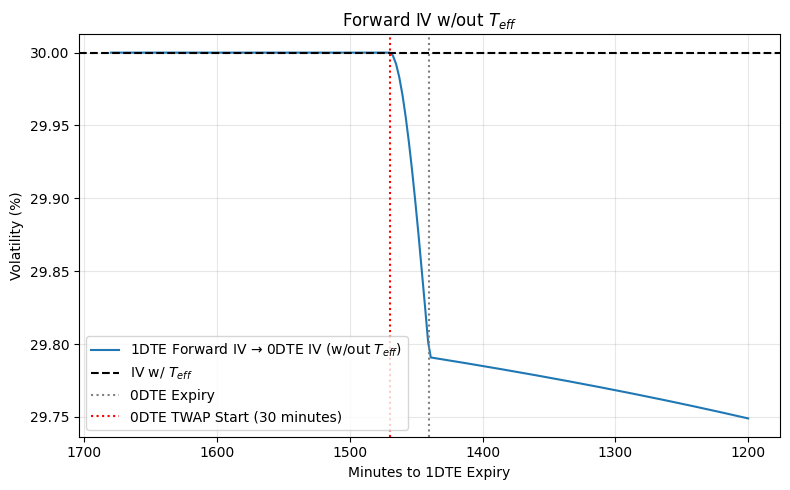
\includegraphics[width=0.5\textwidth]{png3.png}
    \caption{Distortion (kink and decay) in the naively calculated forward volatility $\sigma_{fwd}(T_1, T_2)$ resulting from the artificial decay of the naive spot implied volatility of the TWAP-settled $T_1$ option shown in \Cref{fig:naive_iv_decay}.}
    \label{fig:naive_fwd_vol_kink}
\end{figure}



\subsection{Scenario 2: Naive Market Prices, $T_{\mathrm{eff}}$-Based IV Calculation}

Alternatively, consider if the market (or a specific trader) \textit{ignores} the averaging settlement and prices the option using a standard Black-Scholes model with calendar time $\tau$ and a constant implied volatility $\sigma_{naive}$. If we then analyze these "naive" prices using our theoretically correct \textit{$T_{\mathrm{eff}}$-adjusted model}, we observe the opposite artifact. To reconcile the naive price with the rapidly shrinking $T_{\mathrm{eff}}$ within the averaging window, the implied volatility backed out using the $T_{\mathrm{eff}}$ model must spike dramatically, as shown in \Cref{fig:teff_iv_spike}. This indicates that forcing a constant standard implied volatility onto an average-settled contract leads to prices that are inconsistent with the true variance dynamics near settlement, appearing significantly mispriced from the perspective of the correct model.

\begin{figure}[H]
    \centering
    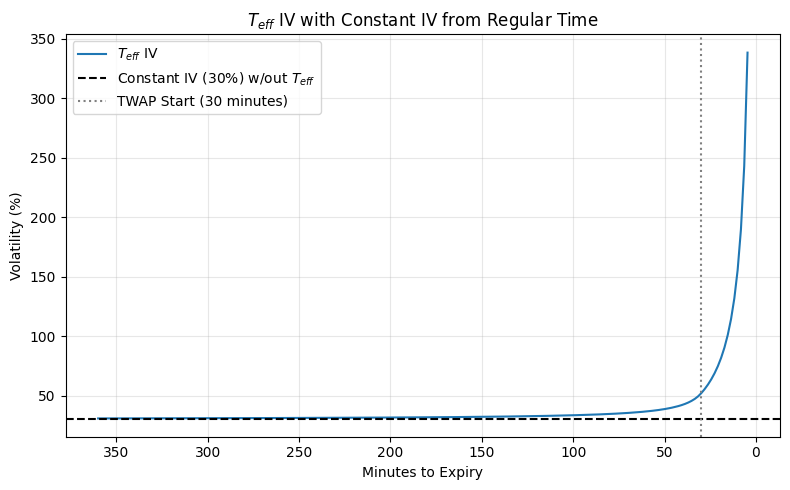
\includegraphics[width=0.5\textwidth]{png4.png}
    \caption{Implied volatility resulting from analyzing naively priced options (ignoring averaging) with the correct $T_{\mathrm{eff}}$-adjusted model. The required volatility spikes unrealistically within the averaging window to match the naive price.}
    \label{fig:teff_iv_spike}
\end{figure}



This scenario also distorts forward volatility. If the $T_1$ option price reflects a naive constant standard implied vol, calculating the forward volatility using the correct $T_{\mathrm{eff}}$ framework for $T_1$ (while still using the standard approach for $T_2$) leads to the spike shown in \Cref{fig:teff_fwd_vol_spike}. This occurs because the variance $V_{correct}(\tau_1)$ implied by the naive price through the $T_{\mathrm{eff}}$ lens becomes excessively large near expiry, distorting the forward variance calculation $V(\tau_2) - V_{correct}(\tau_1)$.

\begin{figure}[H]
    \centering
    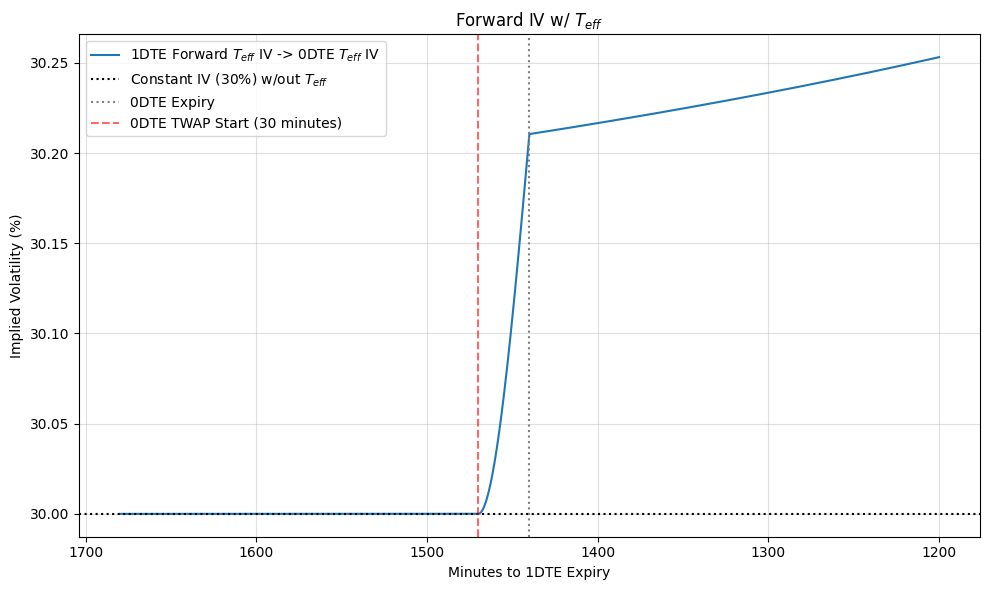
\includegraphics[width=0.5\textwidth]{png5.png}
    \caption{Forward volatility $\sigma_{fwd}(T_1, T_2)$ calculated using the correct $T_{\mathrm{eff}}$ framework for $T_1$, but based on naive market prices for $T_1$ that ignored the averaging effect. The resulting forward volatility spikes and then continues to rise, reflecting the mispricing embedded in the naive $T_1$ price.}
    \label{fig:teff_fwd_vol_spike}
\end{figure}



\subsection{Resolution via $T_{\mathrm{eff}}$}

Both scenarios demonstrate the confusion arising from neglecting the averaging settlement mechanism. The $T_{\mathrm{eff}}$ framework resolves this by providing a model where correctly priced average-settled options exhibit a stable implied volatility (consistent with $\sigma_{true}$) when analyzed with the $T_{\mathrm{eff}}$-adjusted model. This allows for clear interpretation, consistent term structure analysis, meaningful comparisons across different contracts or venues, and avoids attributing structural settlement effects to the volatility parameter.



\section{Conclusion}
\label{sec:conclusion}
This paper addressed the valuation of European options settled on TWAP and VWAP benchmarks within a standard Black-Scholes/Black-76 setting. Recognizing that price averaging reduces effective variance, we derived an adjustment factor, the effective time-to-expiration $T_{\mathrm{eff}}$, based on the variance of the average log-price under GBM. We provided explicit piecewise formulas for $T_{\mathrm{eff}}$ in the TWAP case (\cref{eq:tte_eff_twap}) and derived an explicit closed-form piecewise solution for a VWAP case using a power-law volume profile ($v(s) \propto s^\alpha$, where $s$ is time since window start) over a final averaging window (\cref{eq:tte_eff_vwap_piecewise_final}).

The key contribution is a practical framework that allows practitioners to price these commonly encountered average-settled derivatives using familiar tools, while also providing a consistent lens for interpreting market data. By substituting $T_{\mathrm{eff}}(\tau)$ for $\tau$ specifically in the terms related to volatility ($\sigma^2 T_{\mathrm{eff}}$ and $\sigma \sqrt{T_{\mathrm{eff}}}$) while retaining calendar time $\tau$ for discounting ($e^{-r\tau}$) and drift terms (like $(r-q)\tau$), the method correctly accounts for both the reduced variance from averaging and the full time value of money. As demonstrated, this resolves apparent paradoxes in implied volatility behavior near expiry and stabilizes term structure analysis. Furthermore, this approach offers significant computational advantages over simulation-based methods for routine pricing and risk management, leveraging the efficiency of analytical formulas once $T_{\mathrm{eff}}$ is determined.

Limitations of this study include the reliance on the GBM assumption with constant parameters ($r, \sigma$) and the use of log-price variance as a proxy for the variance related to the arithmetic average settlement price. Furthermore, the VWAP analysis focused on a specific power-law profile ($s^\alpha$ relative to window start) over a fixed window $[T-t_w, T]$, while other profiles and intervals are common in practice and would require specific calculation (potentially involving numerical integration if closed forms are not available).

Future research could extend this framework to incorporate more complex underlying dynamics, such as stochastic volatility or jump-diffusion models. Investigating different, perhaps empirically derived, VWAP weighting functions $w(u)$ and averaging intervals would enhance practical relevance.


\bibliographystyle{plainnat}
\bibliography{bibliography}


\end{document}